\section{New Classification} \label{sec:Serotype_Classification}

Reannotation of the probably false annotated sequences in \autoref{fig:PCA_Clusteree_Knee_4} \textbf{\textsf{C}} as well as increasing of the components in \gls{PCA} successfully raised the accuracy of the pipeline. Thereby new potential ways of \gls{IAV} clustering became possible. Resulting from the improved clustering of segment 4 a new classification involving 56 groups instead of 18 subtypes is proposed (\autoref{fig:Result_Clustertree_Segment_4}).
%neue classification vorschlagen blablabla
% vielleicht bisschen evolution black sea gull etc

\begin{figure}[hbt]
    \centering
    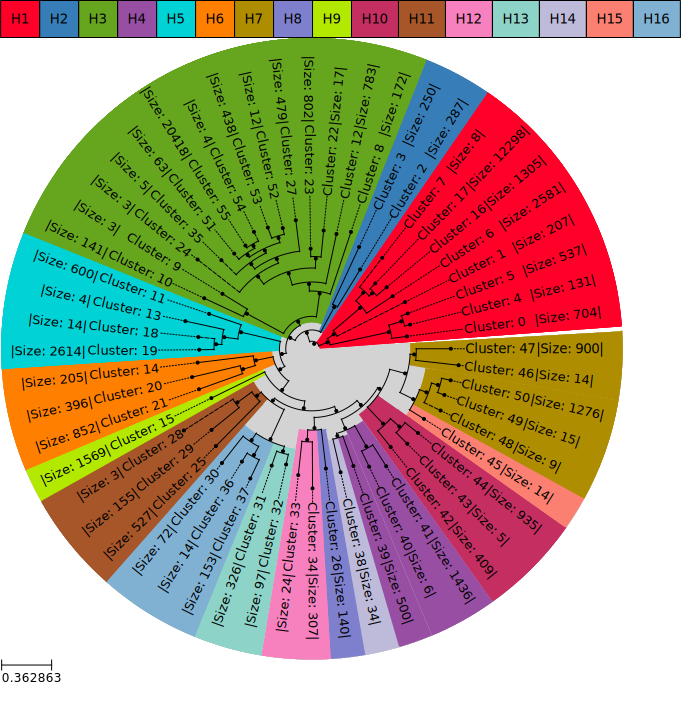
\includegraphics[width=\textwidth]{Results/Clustertree_Segment_4.pdf}
    \caption[]{}
    \label{fig:Result_Clustertree_Segment_4}
\end{figure}

By pairwise comparison of random 10 sequence samples of these groups the similarity inside these groups is described in \autoref{fig:Proof_Clustertree_Segment_4}. To avoid creating a bias, the result for accidental comparisons of sequences with the same accession are ignored and not considered in calculations of respective mean values.

\begin{figure}[hbt]
    \centering
    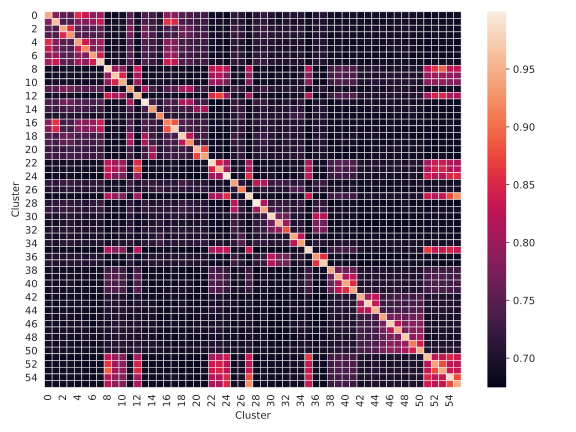
\includegraphics[width=\textwidth]{Results/Cluster_Difference_Segment_4.pdf}
    \caption[]{}
    \label{fig:Proof_Clustertree_Segment_4}
\end{figure}

All clusters in \autoref{fig:Proof_Clustertree_Segment_4} have the highest similarities with themselves and mostly high similarities with clusters of the same subtype. exceptions are the subtypes H7 and H15 with the clusters 45 to 50 as well as H4 and H14 with clusters 35 to 38. There was no clear separation performed as visible in \autoref{fig:Result_Clustertree_Segment_4}. The similarities are high subtype comprehensive and indicate a relation neglected by the subtype classification. 